\setbackground
{
	\centering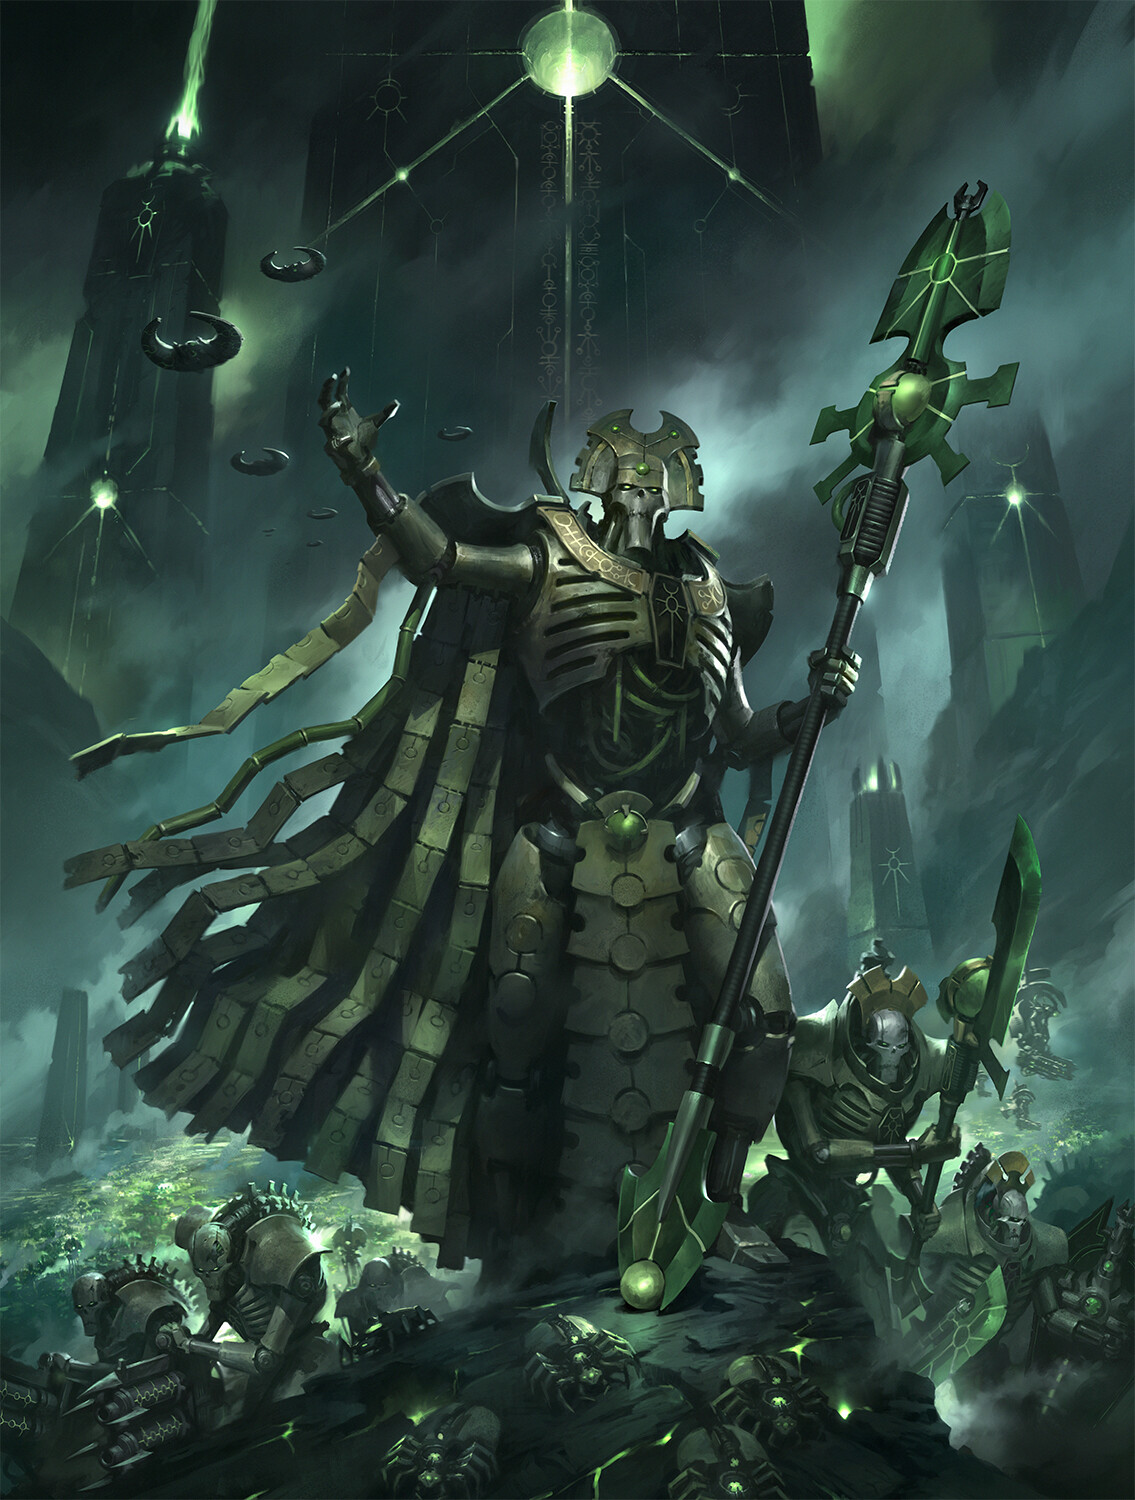
\includegraphics[height=530pt, width=400pt]{hq_art.jpg}
	\subsection[Fast Attack]{\texorpdfstring{\centering\Huge Fast Attack}{Fast Attack}}
	
	\centerline{\begin{minipage}{400pt}
			\centering
			See, Obyron, the separatists come – attempting to outflank me just as they did at the Fourth Battle of Vyndakh. How they calculate that daubing themselves green and roaring like savages will produce a different outcome, I cannot fathom; but it is of no account. Ready my legions – another glorious victory shall soon be ours.
			
			\vspace*{1em}
			\raggedleft Nemesor Zandrekh
	\end{minipage}}
}


\newpage
\clearbackground
\subsubsection[Canoptek Acanthrite Vanguard]{}
\fbox{\begin{imgminipage}{marble.jpg}[t]{0.2\textwidth}
		\color{white}
		\centering {\large FAST ATTACK}
		
		\color{black}
\end{imgminipage}}
\hspace{0.5em}
\begin{minipage}[t]{0.72\textwidth}
	{\large \textbf{Canoptek Acanthrite Vanguard \dotfill X Points}}
	
	\begin{tabular}{m{160 pt} *{10}{c}}
		& M & WS & BS & S & T & W & I & A & Ld & Sv \\
		\hline
		Canoptek Acanthrite & 12 & 4 & 4 & 4 & 5 & 3 & 2 & 2 & 10 & 3+ \\
	\end{tabular}
	\small
	\begin{minipage}[t]{0.5\textwidth}
		\begin{flushleft}
			\vspace*{2em}
			\textbf{Unit Composition}
			\begin{itemize}
				\item 3 Canoptek Acanthrites
			\end{itemize}
			
			\textbf{Wargear}
			\begin{itemize}
				\item \quickref{Cutting Beam}
				\item \quickref{Voidblade}
			\end{itemize}
		\end{flushleft}
	\end{minipage}
	\begin{minipage}[t]{0.5\textwidth}
		\begin{flushleft}
			\vspace*{2em}
			\textbf{Unit Type}
			\begin{itemize}
				\item Infantry (Canoptek, Floating, Light, \quickref{Living Metal})
			\end{itemize}
			
			\textbf{Special Rules}
			\begin{itemize}
				\item \quickref{Annihilation Protocols}
				\item \quickref{Awakening Protocols} (Silver)
				\item Bulky (2)
				\item \quickref{Reanimation Protocols}
				\item Shadowed Wings
				\item \quickref{Soulless Hordes} (Bronze)
			\end{itemize}
		\end{flushleft}
	\end{minipage}
	
	\vspace*{2em}
	\textbf{Weapons}
	
	\begin{tabular}{L{90 pt} c C{40pt} *{2}{c} >{\raggedright\arraybackslash}p{130pt}}
		& Range & Type & S & AP & Abilities \\
		\hline
		Cutting Beam & 12" & Assault 1 & 6 & 2 & Armourbane (Melta) \\
		\quickref{Voidblade} & — & Melee & User & 4 & \quickref{Entropic Strike} (4+), Rending(6+) \\
	\end{tabular}
	
	\vspace*{2em}
	\textbf{Unit Rules}
	
	\textit{Shadowed Wings}: Canoptek Acanthrites increase Shrouded saves by +1. If the model does not already have one, it instead gains Shrouded (6+).
		
	\vspace*{2em}
	\textbf{Options}
	\begin{itemize}
		\item The Canoptek Acanthrites Vanguard may include:
		\begin{itemize}
			\item Up to an additional 6 Canoptek Acanthrites \dotfill X points each
		\end{itemize}
	\end{itemize}
\end{minipage}


\newpage
\subsubsection[Canoptek Scarab Swarms]{}

\begin{minipage}[t]{0.72\textwidth}
	{\large \textbf{Canoptek Scarab Swarms \dotfill 12 Points}}
	
	\begin{tabular}{m{160 pt} *{10}{c}}
		& M & WS & BS & S & T & W & I & A & Ld & Sv \\
		\hline
		Canoptek Scarab Swarm & 10 & 2 & 2 & 3 & 3 & 3 & 2 & 4 & 10 & 6+ \\
	\end{tabular}
	\small
	\begin{minipage}[t]{0.5\textwidth}
		\begin{flushleft}
			\vspace*{2em}
			\textbf{Unit Composition}
			\begin{itemize}
				\item 3 Canoptek Scarab Swarms
			\end{itemize}
			
			\textbf{Wargear}
			\begin{itemize}
				\item Feeder Mandibles
			\end{itemize}
		\end{flushleft}
	\end{minipage}
	\begin{minipage}[t]{0.5\textwidth}
		\begin{flushleft}
			\vspace*{2em}
			\textbf{Unit Type}
			\begin{itemize}
				\item Infantry (Canoptek, Floating, Light, \quickref{Living Metal})
			\end{itemize}
			
			\textbf{Special Rules}
			\begin{itemize}
				\item \quickref{Reanimation Protocols}
				\item Skittering Hordes
				\item \quickref{Soulless Hordes} (Bronze)
				\item Swarms
			\end{itemize}
		\end{flushleft}
	\end{minipage}
	
	\vspace*{2em}
	\textbf{Weapons}
	
	\begin{tabular}{L{90 pt} c C{40pt} *{2}{c} >{\raggedright\arraybackslash}p{130pt}}
		& Range & Type & S & AP & Abilities \\
		\hline
		Feeder Mandible & — & Melee & User & — & \quickref{Entropic Strike} (4+) \\
	\end{tabular}

	\vspace*{2em}
	\textbf{Unit Rules}
	
	\textit{Skittering Hordes:} Models with this special rule that suffer an unsaved Wound with the Instant Death special rule and not the Blast or Template special rule are not immediately removed as a casualty, but instead lose D3 wounds instead of one for each unsaved Wound with the Instant Death special rule inflicted on it.

	\vspace*{2em}
	\textbf{Options}
	\begin{itemize}
		\item The Canoptek Scarab Swarms may include:
		\begin{itemize}
			\item Up to an additional 6 Canoptek Scarab Swarm models \dotfill +4 points each
		\end{itemize}
	\end{itemize}
\end{minipage}
\hspace{0.5em}
\fbox{\begin{imgminipage}{marble.jpg}[t]{0.2\textwidth}
	\color{white}
	\centering {\large FAST ATTACK}
	
	\color{black}
\end{imgminipage}}


\newpage
\subsubsection[Canoptek Spyder Cohort]{}
\fbox{\begin{imgminipage}{marble.jpg}[t]{0.2\textwidth}
		\color{white}
		\centering {\large FAST ATTACK}
		
		\color{black}
\end{imgminipage}}
\hspace{0.5em}
\begin{minipage}[t]{0.72\textwidth}
	{\large \textbf{Canoptek Spyder Cohort \dotfill 40 Points}}
	
	\begin{tabular}{m{160 pt} *{10}{c}}
		& M & WS & BS & S & T & W & I & A & Ld & Sv \\
		\hline
		Canoptek Spyder & 7 & 3 & 3 & 6 & 6 & 3 & 2 & 1 & 10 & 3+ \\
	\end{tabular}
	\small
	\begin{minipage}[t]{0.5\textwidth}
		\begin{flushleft}
			\vspace*{2em}
			\textbf{Unit Composition}
			\begin{itemize}
				\item 1 Canoptek Spyder
			\end{itemize}
			
			\textbf{Wargear}
			\begin{itemize}
				\item Close Combat Weapon
			\end{itemize}
		\end{flushleft}
	\end{minipage}
	\begin{minipage}[t]{0.5\textwidth}
		\begin{flushleft}
			\vspace*{2em}
			\textbf{Unit Type}
			\begin{itemize}
				\item Infantry (Canoptek, Floating, \quickref{Living Metal})
			\end{itemize}
			
			\textbf{Special Rules}
			\begin{itemize}
				\item Bulky (3)
				\item \quickref{Reanimation Protocols}
				\item Nodal Relay
				\item Relentless
				\item Scarab Hive
				\item \quickref{Soulless Hordes} (Silver)
			\end{itemize}
		\end{flushleft}
	\end{minipage}
	
	\vspace*{2em}
	\textbf{Weapons}
	
	\begin{tabular}{L{90 pt} c C{40pt} *{2}{c} >{\raggedright\arraybackslash}p{130pt}}
		& Range & Type & S & AP & Abilities \\
		\hline
		Fabricator Claw Array & — & Melee & User & 5 & — \\
		\quickref{Particle Beamer} & 24" & Heavy 1 & 6 & 5 & Blast, Twin-Linked \\
	\end{tabular}
	
	\vspace*{2em}
	\textbf{Unit Rules}
	
	\textit{Fabricator Claw Array:} Each model with a Fabricator Claw Array gains the Battlesmith (4+) special rule.
	
	\textit{Nodal Relay:} If a Canoptek Spyder is within \quickref{Nodal Range} of a model it will extend that range an additional 6" from the Spyder model, acting as a relay point.
	
	\textit{Scarab Hive:} Once per friendly Movement phase, each Canoptek Spyder model can use this special rule to create Canoptek Scarab Swarms. To do so, nominate a friendly unit of Canoptek Scarab Swarms that is within 6" of the Canoptek Spyder. Add a single Canoptek Scarab Swarm base to the unit – this can take the unit beyond its starting size, but must be placed within 6" of the Canoptek Spyder. If a model cannot be placed for any reason, it is destroyed. Canoptek Scarab Swarms created in this manner can move and act normally this turn. Roll a D6 each time a Canoptek Spyder uses its Scarab Hive special rule, immediately after placing any Canoptek Scarab Swarms that were created – on a roll of a 1 the Canoptek Spyder suffers a single Wound with no saves of any kind allowed. In addition, for each Canoptek Spyder Cohort in the army, a unit of Canoptek Scarab Swarms may be taken which do count towards the maximum number of units in their respective Force Organisation slot.
	
	
	\vspace*{2em}
	\textbf{Options}
	\begin{itemize}
		\item The Canoptek Spyder Cohort may include:
		\begin{itemize}
			\item Up to an additional 2 Canoptek Spyders \dotfill +40 points each
		\end{itemize}
		\item Each model may take replace their Close Combat Weapon with a:
		\begin{itemize}
			\item Fabricator Claw Array \dotfill +5 points each
		\end{itemize}
		\item Each model may take any of the following options:
		\begin{itemize}
		\item \quickref{Gloom Prism} \dotfill +10 points each
		\item Twin-Linked \quickref{Particle Beamer} \dotfill +5 points each
		\end{itemize}
	\end{itemize}
\end{minipage}


\newpage
\subsubsection[Canoptek Tomb Sentinel]{}
\begin{minipage}[t]{0.72\textwidth}
	{\large \textbf{Canoptek Tomb Sentinel \dotfill 100 Points}}
	
	\begin{tabular}{m{160 pt} *{10}{c}}
		& M & WS & BS & S & T & W & I & A & Ld & Sv \\
		\hline
		Canoptek Tomb Sentinel & 10 & 3 & 3 & 6 & 7 & 4 & 2 & 2 & 10 & 3+ \\
	\end{tabular}
	\small
	\begin{minipage}[t]{0.5\textwidth}
		\begin{flushleft}
			\vspace*{2em}
			\textbf{Unit Composition}
			\begin{itemize}
				\item 1 Canoptek Tomb Sentinel
			\end{itemize}
			
			\textbf{Wargear}
			\begin{itemize}
				\item Close Combat Weapon
				\item \quickref{Exile Cannon}
			\end{itemize}
		\end{flushleft}
	\end{minipage}
	\begin{minipage}[t]{0.5\textwidth}
		\begin{flushleft}
			\vspace*{2em}
			\textbf{Unit Type}
			\begin{itemize}
				\item Dreadnought (Canoptek, \quickref{Living Metal})
			\end{itemize}
			
			\textbf{Special Rules}
			\begin{itemize}
				\item Bulky (3)
				\item Outflank
				\item Phase Generator
				\item Phase Tunneling
				\item Rampage (1)
				\item \quickref{Reanimation Protocols}
				\item Sense Clusters
				\item \quickref{Soulless Hordes} (Silver)
				\item Subterranean Assault
				\item \quickref{Tomb Guardians}
			\end{itemize}
		\end{flushleft}
	\end{minipage}
	
	\vspace*{2em}
	\textbf{Weapons}
	
	\begin{tabular}{L{90 pt} c C{40pt} *{2}{c} >{\raggedright\arraybackslash}p{130pt}}
		& Range & Type & S & AP & Abilities \\
		\hline
		\quickref{Exile Cannon} & 12" & Heavy 1 & 10 & 2 & Blast, \quickref{Exile Ray} (5+), Ignores Cover \\
	\end{tabular}
	
	\vspace*{2em}
	\textbf{Unit Rules}
	
	\textit{Phase Generator:} The Canoptek Tomb Sentinel has a 4+ invulnerable save.
	
	\textit{Phase Tunelling:} When moving, a Canoptek Tomb Sentinel can move over all other models and terrain as if they were open ground. However, it cannot end their move on top of other models and can only end their move on top of impassable terrain if it is possible to actually place the models on top of it.
	
	\textit{Sense Clusters:} A Canoptek Tomb Stalker is immune to Blind and has the Night Vision special rule.	
	
	\vspace*{2em}
	\textbf{Options}
	\begin{itemize}
		\item The Canoptek Tomb Stalker may take any of the following options:
		\begin{itemize}
			\item \quickref{Gloom Prism} \dotfill +10 points each
			\item \quickref{Sepulchral Scarabs} \dotfill +10 points each
		\end{itemize}
	\end{itemize}
\end{minipage}
\hspace{0.5em}
\fbox{\begin{imgminipage}{marble.jpg}[t]{0.2\textwidth}
	\color{white}
	\centering {\large FAST ATTACK}
	
	\color{black}
\end{imgminipage}}


\newpage
\subsubsection[Canoptek Tomb Stalker]{}

\fbox{\begin{imgminipage}{marble.jpg}[t]{0.2\textwidth}
		\color{white}
		\centering {\large FAST ATTACK}
		
		\color{black}
\end{imgminipage}}
\hspace{0.5em}
\begin{minipage}[t]{0.72\textwidth}
	{\large \textbf{Canoptek Tomb Stalker \dotfill 85 Points}}
	
	\begin{tabular}{m{160 pt} *{10}{c}}
		& M & WS & BS & S & T & W & I & A & Ld & Sv \\
		\hline
		Canoptek Tomb Stalker & 10 & 3 & 3 & 6 & 7 & 4 & 2 & 4 & 10 & 3+ \\
	\end{tabular}
	\small
	\begin{minipage}[t]{0.5\textwidth}
		\begin{flushleft}
			\vspace*{2em}
			\textbf{Unit Composition}
			\begin{itemize}
				\item 1 Canoptek Tomb Stalker
			\end{itemize}
			
			\textbf{Wargear}
			\begin{itemize}
				\item Two Close Combat Weapons
				\item Two \quickref{Gauss Flayer}s
			\end{itemize}
		\end{flushleft}
	\end{minipage}
	\begin{minipage}[t]{0.5\textwidth}
		\begin{flushleft}
			\vspace*{2em}
			\textbf{Unit Type}
			\begin{itemize}
				\item Dreadnought (Canoptek, Light, \quickref{Living Metal})
			\end{itemize}
			
			\textbf{Special Rules}
			\begin{itemize}
				\item Outflank
				\item Phase Generator
				\item Phase Tunneling
				\item Rampage (1)
				\item \quickref{Reanimation Protocols}
				\item Sense Clusters
				\item \quickref{Soulles Hordes} (Silver)
				\item Subterranean Assault
				\item \quickref{Tomb Guardians}
			\end{itemize}
		\end{flushleft}
	\end{minipage}
	
	\vspace*{2em}
	\textbf{Weapons}
	
	\begin{tabular}{L{90 pt} c C{40pt} *{2}{c} >{\raggedright\arraybackslash}p{130pt}}
		& Range & Type & S & AP & Abilities \\
		\hline
		\quickref{Gauss Flayer} & 24" & Rapid Fire & 4 & 5 & \quickref{Gauss} (6+) \\
	\end{tabular}
	
	\vspace*{2em}
	\textbf{Unit Rules}
	
	\textit{Phase Generator:} The Canoptek Tomb Sentinel has a 4+ invulnerable save.
	
	\textit{Phase Tunelling:} When moving, a Canoptek Tomb Sentinel can move over all other models and terrain as if they were open ground. However, it cannot end their move on top of other models and can only end their move on top of impassable terrain if it is possible to actually place the models on top of it.
	
	\textit{Sense Clusters:} A Canoptek Tomb Stalker is immune to Blind and has the Night Vision special rule.	
	
	\vspace*{2em}
	\textbf{Options}
	\begin{itemize}
		\item The Canoptek Tomb Stalker may take any of the following options:
		\begin{itemize}
			\item \quickref{Gloom Prism} \dotfill +10 points each
			\item \quickref{Sepulchral Scarabs} \dotfill +10 points each
		\end{itemize}
	\end{itemize}
\end{minipage}




\newpage
\subsubsection[Canoptek Wraith Flight]{}

\fbox{\begin{imgminipage}{marble.jpg}[t]{0.2\textwidth}
		\color{white}
		\centering {\large FAST ATTACK}
		
		\color{black}
\end{imgminipage}}
\hspace{0.5em}
\begin{minipage}[t]{0.72\textwidth}
	{\large \textbf{Canoptek Wraith Flight \dotfill X Points}}
	
	\begin{tabular}{m{160 pt} *{10}{c}}
		& M & WS & BS & S & T & W & I & A & Ld & Sv \\
		\hline
		Canoptek Wraith & 12 & 3 & 3 & 4 & 5 & 2 & 2 & 3 & 10 & 3+ \\
	\end{tabular}
	\small
	\begin{minipage}[t]{0.5\textwidth}
		\begin{flushleft}
			\vspace*{2em}
			\textbf{Unit Composition}
			\begin{itemize}
				\item 3 Canoptek Wraiths
			\end{itemize}
			
			\textbf{Wargear}
			\begin{itemize}
				\item Close Combat Weapon
			\end{itemize}
		\end{flushleft}
	\end{minipage}
	\begin{minipage}[t]{0.5\textwidth}
		\begin{flushleft}
			\vspace*{2em}
			\textbf{Unit Type}
			\begin{itemize}
				\item Infantry (Canoptek, Light, \quickref{Living Metal})
			\end{itemize}
			
			\textbf{Special Rules}
			\begin{itemize}
				\item Bulky (3)
				\item \quickref{Reanimation Protocols}
				\item \quickref{Soulless Hordes} (Silver)
				\item Wraithform
				\item Wraithflight
			\end{itemize}
		\end{flushleft}
	\end{minipage}
	
	\vspace*{2em}
	\textbf{Weapons}
	
	\begin{tabular}{L{90 pt} c C{40pt} *{2}{c} >{\raggedright\arraybackslash}p{130pt}}
		& Range & Type & S & AP & Abilities \\
		\hline
		\quickref{Whip Coils} & — & Melee & User & — & Reach (3) \\
		\quickref{Particle Caster} & 12" & Pistol 1 & 6 & 5 & — \\
		\quickref{Transdimensional Beamer} & 12" & Heavy 1 & 4 & 5 & \quickref{Exile Ray} (6+) \\
	\end{tabular}
	
	\vspace*{2em}
	\textbf{Unit Rules}
	
	\textit{Wraithform:} Each Canoptek Wraith has a 3+ invulnerable save.
	
	\textit{Wraithflight:} When moving, a Canoptek Wraith can move over all other models and terrain as if they were open ground. However, it cannot end their move on top of other models and can only end their move on top of impassable terrain if it is possible to actually place the models on top of it.	
	
	\vspace*{2em}
	\textbf{Options}
	\begin{itemize}
		\item The Canoptek Wraith Flight may include:
		\begin{itemize}
			\item Up to an additional 3 Canoptek Wraiths \dotfill X points each
		\end{itemize}
		\item Each model may take exchange their Close Combat Weapon for:
		\begin{itemize}
			\item \quickref{Whip Coils} \dotfill X points each
		\end{itemize}
		\item Each model may take one of the following options:
		\begin{itemize}
			\item \quickref{Particle Caster} \dotfill X points each
			\item \quickref{Transdimensional Beamer} \dotfill X points each
		\end{itemize}
	\end{itemize}
\end{minipage}


\newpage
\subsubsection[Ghost Ark]{}
\fbox{\begin{imgminipage}{marble.jpg}[t]{0.2\textwidth}
		\color{white}
		\centering {\large Fast Attack}
		
		\raggedright \small
		\color{black}
\end{imgminipage}}
\hspace{0.5em}
\begin{minipage}[t]{0.72\textwidth}
	{\large \textbf{Ghost Ark \dotfill 100 Points}}
	\begin{NiceTabular}{m{145 pt} *{2}{c} | *{3}{c} | c | c }
		& & & \cellgray{3}{Armour} & & & & \cellgray{1}{Transport} \\
		& M & BS & \cellgray{1}{Front} & \cellgray{1}{Side} & \cellgray{1}{Rear} & HP & \cellgray{1}{Capacity} \\
		\hline
		Ghost Ark & 12 & 4 & \cellgray{1}{11} & \cellgray{1}{11} & \cellgray{1}{11} & 4 &\cellgray{1}{11} \\
	\end{NiceTabular}
	\small
	\begin{minipage}[t]{0.5\textwidth}
		\begin{flushleft}
			\vspace*{2em}
			\textbf{Unit Composition}
			\begin{itemize}
				\item 1 Ghost Ark
			\end{itemize}
			
			\textbf{Wargear}
			\begin{itemize}
				\item Five Sponson (Left) Mounted \quickref{Gauss Flayer}s
				\item Five Sponson (Right) Mounted \quickref{Gauss Flayer}s
				\item \quickref{Quantum Shielding}
			\end{itemize}
		\end{flushleft}
	\end{minipage}
	\begin{minipage}[t]{0.5\textwidth}
		\begin{flushleft}
			\vspace*{2em}
			\textbf{Unit Type}
			\begin{itemize}
				\item Vehicle (\quickref{Living Metal}, Open-Topped, Skimmer, Transport)
			\end{itemize}
			
			\textbf{Special Rules}
			\begin{itemize}
				\item \quickref{Awakening Protocols} (Bronze)
				\item Power of the Machine Spirit
			\end{itemize}
		\end{flushleft}
	\end{minipage}

	\vspace*{2em}
	\textbf{Access Points}
	
	The Ghost Ark has three Access Points on the Front and Sides of the hull.
	
	\vspace*{2em}
	\textbf{Weapons}
	
	\begin{tabular}{L{90 pt} c C{40pt} *{2}{c} >{\raggedright\arraybackslash}p{130pt}}
		& Range & Type & S & AP & Abilities \\
		\hline
		\quickref{Gauss Flayer} & 24" & Rapid Fire & 4 & 5 & \quickref{Gauss} (6+) \\
	\end{tabular}
	
	\vspace*{2em}
	\textbf{Unit Rules}
	
	\textit{Repair Barge}: At the start of each friendly Movement phase, this model can repair fallen Dynastic Warriors. To do so, nominate a friendly unit of Dynastic Warriors that is either within 6" of this model or embarked upon it, and roll a D3: that unit reanimate that may times; if embarked, this cannot return models above the Transport Capacity. These Dynastic Warriors must be placed within 6" of the Ghost Ark, or if the unit is currently embarked in the Ghost Ark, within it. If a model cannot be placed for any reason, it is destroyed. Dynastic Warriors repaired in this manner can move and act normally this turn. 
	
	
	\vspace*{2em}
	\textbf{Options}
	\begin{itemize}
	\item A Ghost Ark may take:
	\begin{itemize}
		\item \quickref{Quantum Shielding Matrix} \dotfill +5 points
	\end{itemize} 
	\end{itemize} 
\end{minipage}



\newpage
\subsubsection[Night Scythe]{}
\fbox{\begin{imgminipage}{marble.jpg}[t]{0.2\textwidth}
		\color{white}
		\centering {\large Fast Attack}
		
		\raggedright \small
		\color{black}
\end{imgminipage}}
\hspace{0.5em}
\begin{minipage}[t]{0.72\textwidth}
	{\large \textbf{Night Scythe \dotfill 105 Points}}
	\begin{NiceTabular}{m{145 pt} *{2}{c} | *{3}{c} | c | c }
		& & & \cellgray{3}{Armour} & & & & \cellgray{1}{Transport} \\
		& M & BS & \cellgray{1}{Front} & \cellgray{1}{Side} & \cellgray{1}{Rear} & HP & \cellgray{1}{Capacity} \\
		\hline
		Night Scythe & 24 & 4 & \cellgray{1}{11} & \cellgray{1}{11} & \cellgray{1}{11} & 4 &\cellgray{1}{—} \\
	\end{NiceTabular}
	\small
	\begin{minipage}[t]{0.5\textwidth}
		\begin{flushleft}
			\vspace*{2em}
			\textbf{Unit Composition}
			\begin{itemize}
				\item 1 Night Scythe
			\end{itemize}
			
			\textbf{Wargear}
			\begin{itemize}
				\item Hull (Front) Mounted Twin-Linked \quickref{Tesla Destructor}
				\item Captive Wormhole
			\end{itemize}
		\end{flushleft}
	\end{minipage}
	\begin{minipage}[t]{0.5\textwidth}
		\begin{flushleft}
			\vspace*{2em}
			\textbf{Unit Type}
			\begin{itemize}
				\item Vehicle (Hover, Flyer, \quickref{Living Metal}, Transport)
			\end{itemize}
			
			\textbf{Special Rules}
			\begin{itemize}
				\item \quickref{Awakening Protocols} (Bronze)
				\item Invasion Beams
			\end{itemize}
		\end{flushleft}
	\end{minipage}
	
	\vspace*{2em}
	\textbf{Access Points}
	
	The Night Scythe has one Access Point on each side of the hull.
	
	\vspace*{2em}
	\textbf{Weapons}
	
	\begin{tabular}{L{90 pt} c C{40pt} *{2}{c} >{\raggedright\arraybackslash}p{130pt}}
		& Range & Type & S & AP & Abilities \\
		\hline
		\quickref{Tesla Destructor} & 36" & Heavy 4 & 7 & — & \quickref{Tesla} (6+), Twin-Linked
	\end{tabular}
	
	\vspace*{2em}
	\textbf{Unit Rules}
	
	\textit{Captive Wormhole:} A Night Scythe does not have a traditional Transport Capacity. Instead, units embarked on the it are \textbf{stationed} at its Captive Wormhole. The stationed unit may exit the Night Scythe using any of the normal Transport rules, however they are never affected by anything that affects Passengers and do not count as being embarked for the purposes of special rules or effects. While the unit is stationed at the Captive Wormhole, they also count as being in \quickref{Teleportation Reserves}; should the Night Scythe be destroyed, the stationed unit is not affected and goes into \quickref{Teleportation Reserves}. A unit that embarks the Night Scythe are sent to the Captive Wormhole and count as being stationed at the Captive Wormhole. A Night Scythe can only have a single unit stationed at its Captive Wormhole at any given time.
	
	\textit{Invasion Beams}: A unit that begins its Movement phase embarked upon a Night Scythe can disembark either before or after it has moved (including pivoting on the spot), even though it is Zooming, so long it has not moved more than 36" in that Movement phase. If a unit disembarks from a Night Scythe after it has moved 24" or more, models in the unit can only fire Snap Shots until the start of their next turn.
\end{minipage}


\newpage
\subsubsection[Tomb Blade Wing]{}

\fbox{\begin{imgminipage}{marble.jpg}[t]{0.2\textwidth}
		\color{white}
		\centering {\large FAST ATTACK}
		
		\color{black}
\end{imgminipage}}
\hspace{0.5em}
\begin{minipage}[t]{0.72\textwidth}
	{\large \textbf{Tomb Blade Wing \dotfill X Points}}
	
	\begin{tabular}{m{160 pt} *{10}{c}}
		& M & WS & BS & S & T & W & I & A & Ld & Sv \\
		\hline
		Tomb Blade & 16 & 4 & 4 & 4 & 5 & 2 & 2 & 1 & 10 & 4+ \\
	\end{tabular}
	\small
	\begin{minipage}[t]{0.5\textwidth}
		\begin{flushleft}
			\vspace*{2em}
			\textbf{Unit Composition}
			\begin{itemize}
				\item 3 Tomb Blades
			\end{itemize}
			
			\textbf{Wargear}
			\begin{itemize}
				\item Twin-Linked \quickref{Gauss Blaster}
			\end{itemize}
		\end{flushleft}
	\end{minipage}
	\begin{minipage}[t]{0.5\textwidth}
		\begin{flushleft}
			\vspace*{2em}
			\textbf{Unit Type}
			\begin{itemize}
				\item Cavalry (Floating, \quickref{Living Metal}, Skirmish)
			\end{itemize}
			
			\textbf{Special Rules}
			\begin{itemize}
				\item \quickref{Awakening Protocols} (Silver)
				\item Bulky (3)
				\item Hammer of Wrath (1)
				\item Hit \& Run
				\item Outflank
				\item \quickref{Reanimation Protocols}
				\item Relentless
			\end{itemize}
		\end{flushleft}
	\end{minipage}
	
	\vspace*{2em}
	\textbf{Weapons}
	
	\begin{tabular}{L{90 pt} c C{40pt} *{2}{c} >{\raggedright\arraybackslash}p{130pt}}
		& Range & Type & S & AP & Abilities \\
		\hline
		\quickref{Gauss Blaster} & 24" & Rapid Fire & 5 & 4 & \quickref{Gauss} (6+), Twin-Linked \\
		\quickref{Tesla Carbine} & 24" & Assault 2 & 5 & — & \quickref{Tesla} (6+), Twin-Linked \\
		\quickref{Particle Beamer} & 24" & Heavy 1 & 6 & 5 & Blast \\
	\end{tabular}
	
	\vspace*{2em}
	\textbf{Unit Rules}
	
	\textit{Nebuloscope}: A model with a Nebuloscope gains the Night Vision special rule and their weapons gain the Ignores Cover special rule.
	
	\textit{Shadowloom}: A model with a Shadowloom increases Shrouded saves by +1. If it does not already have one, it instead gains Shrouded (6+).
	
	\textit{Shieldvane}: A model with a Shieldvane increases their save to 3+.
	
	\vspace*{2em}
	\textbf{Options}
	\begin{itemize}
		\item The Tomb Blade Wing may include:
		\begin{itemize}
			\item Up to an additional 7 Tomb Blades \dotfill X points each
		\end{itemize}
		\item Each Tomb Blade make take any of the following options:
		\begin{itemize}
			\item \quickref{Nebuloscope} \dotfill X points each
			\item \quickref{Shadowloom} \dotfill X points each
			\item \quickref{Shieldvane} \dotfill X points each
		\end{itemize}
		\item Each Tomb Blade may exchange their Twin-Linked \quickref{Gauss Blaster} for one of the following:
		\begin{itemize}
			\item Twin-Linked \quickref{Tesla Carbine} \dotfill X points each
			\item \quickref{Particle Beamer} \dotfill X points each
		\end{itemize}
	\end{itemize}
\end{minipage}